\section{Experiments}
\label{sec:experiment}
In this section, we first present dataset and evaluation metrics used in our experiments. Then we investigate several design choices of our framework 
and compare them against previous methods.

\subsection{Dataset}
\label{sec:data}

Our MCQ dataset covers multiple domains including science,  
vocabulary, common sense and trivia.
It is compiled from a wide variety of open source  
MCQ dataset including SciQ~\cite{welbl2017crowdsourcing}, 
MCQL~\cite{liang2018distractor}, AI2 Science Questions as well as trivia, and 
vocabulary MCQs crawled from websites. 
We filter out MCQs whose keys are not short phrases since this paper only 
focuses on extractive cloze-style DG, resulting in 2,880 items in total among which 1176 are from SciQ, 300 are from MCQL, 275 are from AI2 and the rest from website resources.
Statistics of the dataset are summarized in \tabref{table:dataset} and \figref{fig:pos}.
% Table \ref{table:dataset} summarizes the statistics of our dataset. The part-of-speech (POS) distributions of the keys are also presented in \figref{fig:pos}.
% \begin{figure*}[t!]
% 	\vspace{-0.4cm}
% 	\begin{minipage}[b]{0.5\linewidth}
% 		\centering
% 		\includegraphics[width=1.0\columnwidth]{figure/dist.eps}
% 		\caption{POS distribution of keys.}
% 		\label{fig:pos}
% 	\end{minipage}%
% 	\begin{minipage}[b]{0.5\linewidth}
% 		\centering
% 		\small
% 		\addtolength{\tabcolsep}{-2pt}
% 		\begin{tabular}{l|c|cccc}
% 		\toprule
% 		\multirow{2}{*}{Domain} & \multirow{2}{*}{Total} & \multirow{2}{*}{Science} & \multirow{2}{*}{Vocab.} & \multirow{2}{*}{\shortstack{Common\\Sense}} & \multirow{2}{*}{Trivia}\\
% 		& & & & & \\
% 		\midrule
% 		\# MCQs & 2880 & 758 & 956 & 706 & 460\\
% 		\midrule
% 		\# Distractors & 3.13 & 3.00 & 3.99 & 3.48 & 2.99\\
% 		\bottomrule
% 	\end{tabular}
% 	\caption{Dataset Statistics (number of MCQs in each domain and average number of distractors per question)}
% 	\label{table:dataset}
% 	\end{minipage}%	
% \end{figure*}



% \begin{table}[thb!]
% \small
% \addtolength{\tabcolsep}{-2pt}
% \centering
% 	\begin{tabular}{l|c|cccc}
% 		\toprule
% 		\multirow{2}{*}{Domain} & \multirow{2}{*}{Total} & \multirow{2}{*}{Science} & \multirow{2}{*}{Vocab.} & \multirow{2}{*}{\shortstack{Common\\Sense}} & \multirow{2}{*}{Trivia}\\
% 		& & & & & \\
% 		\midrule
% 		\# MCQs & 2880 & 758 & 956 & 706 & 460\\
% 		\midrule
% 		\# Distractors & 3.13 & 3.00 & 3.99 & 3.48 & 2.99\\
% 		\bottomrule
% 	\end{tabular}
% 	\caption{Dataset Statistics (number of MCQs in each domain and average number of distractors per question)}
% 	\label{table:dataset}
% \end{table}
% \begin{figure}[htb!]
% 	\centering
% 	\scalebox{0.5}{\includegraphics[width=1.0\columnwidth]{figure/dist.eps}}
% 	\caption{Part-of-speech distribution of keys in different domains.} \label{fig:pos}
% \end{figure}
We convert questions to cloze form by constructing Penn Treebank style trees using Stanford Parser~\cite{klein2003accurate}, and adjusting node order according to the identified question type. The dataset is randomly devided into train/valid/test with a ratio of 8:1:1.
We use the tokenizer and POS tagger from NLTK~\cite{Loper:2002:NNL:1118108.1118117} to preprocess the stems and keys when constructing features.
\begin{table}[ht!]
	\vspace{-0.4cm}
	\centering
	\small
	\addtolength{\tabcolsep}{-2pt}
	\begin{tabular}{l|c|cccc}
	\toprule
	\multirow{2}{*}{Domain} & \multirow{2}{*}{Total} & \multirow{2}{*}{Science} & \multirow{2}{*}{Vocab.} & \multirow{2}{*}{\shortstack{Common\\Sense}} & \multirow{2}{*}{Trivia}\\
	& & & & & \\
	\midrule
	\# MCQs & 2880 & 758 & 956 & 706 & 460\\
	\midrule
	\# Distractors & 3.13 & 3.00 & 3.99 & 3.48 & 2.99\\
	\bottomrule
	\end{tabular}
\caption{Dataset Statistics (number of MCQs in each domain and average number of distractors per question)}
\label{table:dataset}
\end{table}
\begin{figure}[ht!]
	 	\centering
 		\includegraphics[width=1.0\columnwidth]{figure/dist.eps}
 		\caption{POS distribution of keys.}
 		\label{fig:pos}
\end{figure}
\subsection{Evaluation Metrics}
\label{sec:metrics}
% We use the following metrics to evaluate distractor generation methods:
\textbf{Automatic Evaluation.} ~Following~\cite{liang2018distractor}, we report F1 score(F1@3), 
precision(P@1, P@3) and recall~(R@3) to show how well the generated distractors 
match the ground truth distractors, 
as well as the mean reciprocal rank (MRR) and normalized discounted 
cumulative gain (NDCG@10). Sometimes the generated distractors
do not exactly match the ground truth, but are semantically very close. 
Word2vec model trained on Wikipedia dump 
is utilized to measure the averaged cosine similarity~(Semantic Similarity@3) between top three generated 
distractors and ground truth distractors.  

\noindent
\textbf{Human Evaluation.} ~Following~\cite{jiang2017distractor}, we ask three proficient English speakers to evaluate distractors' reliability and plausibility by showing them the key. We evenly sample 50 items in all domains from test set, each item contains multiple distractors including 3 generated by each method and all ground truth distractors 
designed by human experts. For each distractor, the judges decided whether 
it is correct or incorrect given the context. For a distractor deemed to 
be incorrect, the reliability score is 1 and the judges further assess 
its plausibility on a 3-point scale: 
``Obviously Wrong'' (0 point), 
``Somewhat Plausible'' (1 point), 
or ``Plausible'' (2 points). We then conduct application-centric evaluation using another 50 samples without keys from test set by extending original sample with additionally generated distractors and asking testees to answer it. Results are included in \secref{sec:res}.


% \textbf{Ranking Measures} 
% % To some extent, whether the ground truth distractors 
% % come out on the top of the result list demonstrate the effectiveness of 
% % the distractor generator. 
% Following~\cite{liang2018distractor}, we report top F1 score(F1@3), 
% precision(P@1, P@3) and recall~(R@3) to show how well the generated distractors 
% match the ground truth distractors, 
% as well as the mean reciprocal rank (MRR) and normalized discounted 
% cumulative gain (NDCG@10) to show the positions of ground truth distractors 
% in the output ranked list. 
% % Intuitively, we consider the ground truth distractors designed by human experts as good distractors.  

% \textbf{Semantic Similarity} Sometimes the generated distractors
% do not exactly match the ground truth, but are semantically very close. 
% Word2vec~\cite{mikolov2013distributed} model trained on Wikipedia dump 
% is utilized to measure the averaged cosine similarity~(Semantic Similarity@3) between top three generated 
% distractors and ground truth distractors. 

\subsection{Design Choices of CSG and DS}
\label{sec:ablation}

We investigate Probase and WordNet as the knowledge base in CSG and additionally extract all words and phrases from WordNet as a baseline of CSG in following experiments. For Probase, both $p(c|a)$ and $p(d|c)$ are natively supported and can be obtained using official APIs. Size of concept set $C$ is set to be 20. For nouns and verbs in WordNet, we treat the set of unique hypernyms~(as well as their siblings) of all synsets for $a$ as concept set $C$ and compute
$p(c|a)$ using the Laplace-smoothed Bayes rule on the lemma frequency provided in WordNet~(count on sense tagged text). We choose all synsets and their similar/antonymic sets as concept set $C$ for adjectives and adverbs in WordNet. Topic distributions $\pi_{a,q}$ and $\gamma_c$ are obtained using LDA pre-trained on Wikipedia dump and $K$ is set to 100.

% \subsubsection*{Instantiation of DS}
% As mentioned before in \secref{sec:DS}, one can customize DS with various learning-to-rank model. 
For DS, we experiment with point-wise, pair-wise and list-wise ranking models to find the best practice.
Specifically, we employ AdaBoost~\cite{freund1997decision} as point-wise ranker and LambdaMART~\cite{burges2010from} as both pair-wise and list-wise ranker. The dimensionality of feature vector $l$ is 33. Unigram frequency is calculated on Wikipedia dump. For the training of DS, negative examples are sampled using top 100 candidates extracted by CSG excluding those that are within ground truths. At test time, DS takes as input top 30 candidates extracted by CSG 
and 30 candidates sampled from WordNet's own vocabulary having the same POS tag. All hyperparameters are tuned on dev set.



\subsection{Baselines}
We name our framework \textbf{CSG+DS} and compare it against the following baselines:
\begin{itemize}
%	\setlength{\itemsep}{1pt}
%	\setlength{\parsep}{1pt}
%	\setlength{\parskip}{1pt}
	\item \textit{Thesaurus-based Method (TM)}~\cite{sumita2005measuring} ranks candidate distractors from synonyms of the key in WordNet based on path similarity and applys post-filtering via IR.
	\item \textit{RevUP}~\cite{Kumar2015RevUP} ranks candidate distractors based on weighted average of word2vec similarity, dice coefficient and language model probability.
	\item \textit{EmbSim+CF}~\cite{jiang2017distractor} combines word2vec similarity, tri-gram and dependency candidate filtering in ranking and filtering respectively.
	\item \textit{ED} use edit distance to measure the spelling similarity between distractors and key.

	\item \textit{LR+RF}~\cite{liang2018distractor} combines logistic regression and random forest as a two-stage cascaded ranker with features measuring the plausibility of distractors.
	\item \textit{LR+LM}~\cite{liang2018distractor} replaces random forest in LR+RF with LambdaMART.
	% \item \textit{BERT}~\cite{devlin2018bert} predicts blank gap in the stem as distractors based on contextual information.
	\item \textit{BERT}~\cite{Wolf2019HuggingFacesTS} ranks candidates based on cosine similarity of their BERT embeddings with that of the key.
\end{itemize}
Trigram and 5-gram Kneser Ney language model are built upon the original corpus of our dataset. Word2Vec~(CBOW) is pre-trained on Wikipedia dump and fine-tuned on our corpus. Dependency parsing tree is obtained using Spacy toolkit~\cite{spacy2}. We fetch the uncased base version of BERT and fine-tune it on our corpus.
\begin{table*}[t!]
	\small
	\centering
	\vspace{-0.4cm}
	\begin{tabular}{cc c c c c c c c}
		\toprule
		\multicolumn{2}{c}{\textbf{Instantiation}} &\multirow{2}{*}{F1@3} &\multirow{2}{*}{P@1} &\multirow{2}{*}{P@3} &\multirow{2}{*}{R@3} &\multirow{2}{*}{MRR} &\multirow{2}{*}{NDCG@10} &\multirow{2}{*}{\tabincell{c}{Semantic \\Similarity@3}} \\
		\\ [-1.8ex]
		\cline{1-2}
		\\ [-1.8ex]
		CSG &DS & & & & & & &\\
		\midrule
		\multirow{4}{*}{WordNet} &- &3.14 &3.49 &2.33 &5.43 &7.19 &8.66 &0.27 \\
		&point-wise ranker &7.26 &9.30 &5.55 &11.95 &14.30 &14.63 &0.36 \\
		&pair-wise ranker &7.11 &\textbf{10.07} &5.30 &12.14  &\textbf{14.40} &14.84 &0.35 \\
		&list-wise ranker &\textbf{7.71} &9.31 &\textbf{5.81} &\textbf{12.98} &14.34 &\textbf{14.94} &\textbf{0.36} \\
		\midrule
		\multirow{4}{*}{Probase} &- &5.88 &6.98 &4.39 &9.95  &12.07 &13.40 &0.35 \\
		&point-wise ranker &7.91 &8.14 &5.94 &12.98  &15.09 &17.69 &0.41 \\	
		&pair-wise ranker &\textbf{9.42} &10.08 &\textbf{7.00} &15.88  &17.33 &\textbf{19.70} &0.40 \\
		&list-wise ranker &9.19 &\textbf{10.85} &6.72 &\textbf{15.88}  &\textbf{17.51} &19.31 &\textbf{0.41} \\
		\midrule
		\multirow{4}{*}{w/o CSG} &- &- &- &- &- &- &- &- \\
		&point-wise ranker &5.59 &4.63 &3.98 &10.29 &8.67 &11.02 &0.36 \\
		&pair-wise ranker &5.62 &\textbf{5.01} &3.98 &10.10  &\textbf{9.28} &\textbf{11.60} &\textbf{0.36} \\
		&list-wise ranker &\textbf{5.94} &4.24 &\textbf{4.24} &\textbf{10.81} &8.81 &11.46 &0.35 \\
		\bottomrule
	\end{tabular}
	\caption{Comparison of combinations of different choices of CSG and DS. - means no ranking.}
	\label{table:instantiations}
\end{table*}
\begin{figure}[ht]
		\centering
		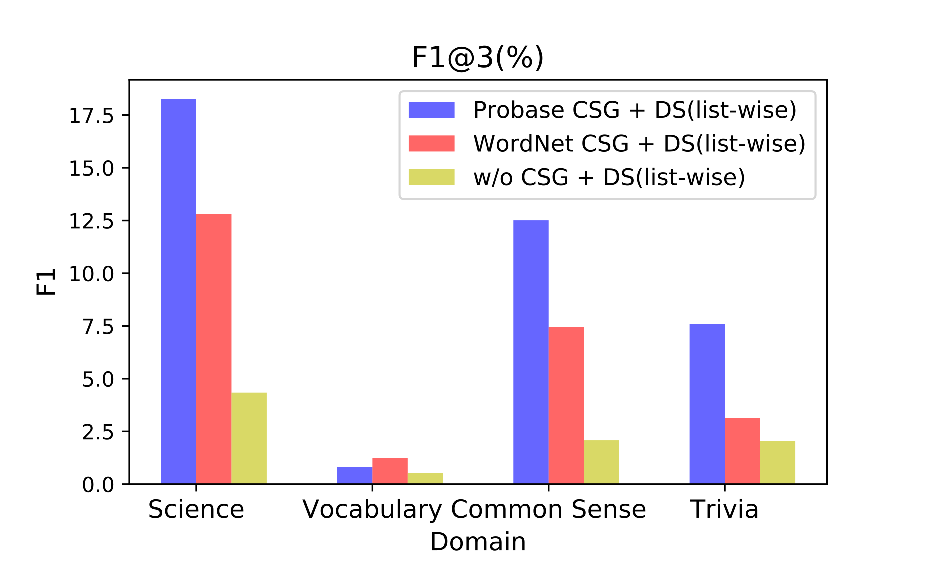
\includegraphics[width=1\columnwidth]{figure/f1.eps}
		\caption{F1@3 score in different domains.}
		\label{fig:domains}
\end{figure}

%\begin{figure*}[t!]
%	\small
%	\vspace{-0.4cm}
%	\begin{minipage}[b]{0.5\linewidth}
%		\centering
%		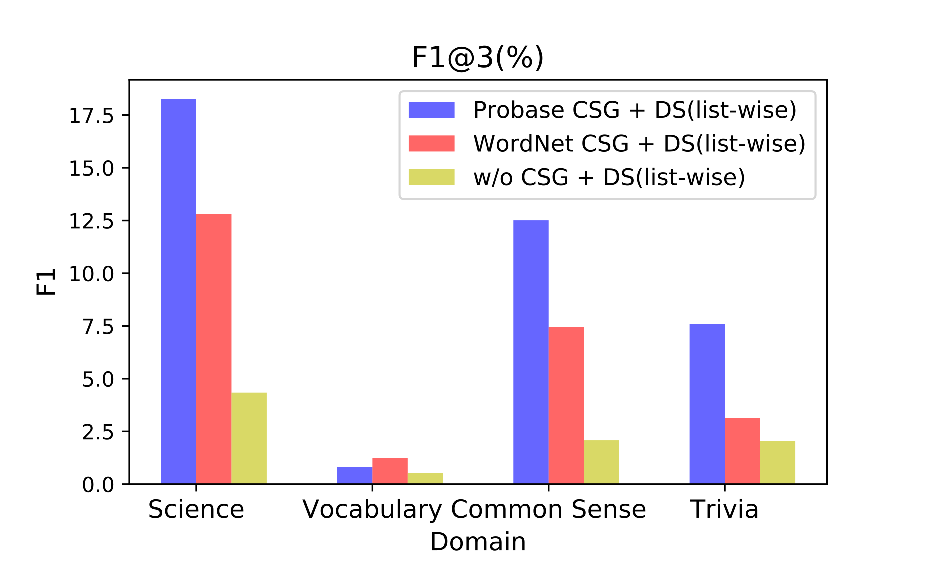
\includegraphics[width=1\columnwidth]{figure/f1.eps}
%		\caption{F1@3 score in different domains.}
%		\label{fig:domains}
%	\end{minipage}%
%	\begin{minipage}[b]{0.5\linewidth}
%		\centering
%		\small
%		\addtolength{\tabcolsep}{-2pt}
%		\begin{tabular}{c|c}
%		\toprule
%		Probase CSG & WordNet CSG \\
%
%			\midrule
%		contextual embed sim(a,d) & contextual embed sim(a,d) \\
%		 word2vec embed sim(a,d)   & word2vec embed sim(a,d)  \\
%		  word2vec embed sim(q,d)& word2vec embed sim(q,d)  \\
%		  web search score & web search score \\
%		  relative LCS len(d)   & relative LCS len(d)  \\
%		  relative LCS len(a)  & relative LCS len(a)  \\
%		  character len(d)   & character len(d)  \\
%		  character len difference(a,d)   & character len difference(a,d)  \\
%		  edit distance(a,d)   & edit distance(a,d)  \\
%		  POS similarity(a,d)   &  relative common suffix len(a) \\
%		\bottomrule
%	\end{tabular}
%	\caption{Top 10 important features of list-wise DS.}
%	\label{table:feat_importance}
%	\end{minipage}%	
%\end{figure*}
\subsection{Results \& Analysis}
\label{sec:res}

% Most baselines we compare to are built upon various knowledge base or fixed vocabulary(denoted in the legend).~Hence, we first examine the capacity of different candidate sources by calculating the recall without re-ranking step\footnote{Candidate filtering in TM, word2vec similarity in WP and BERT+WS.}.~\tabref{table:recall} summarizes the average Recall@K of CSG, BERT\footnote{BERT+WS without re-ranking is identital to BERT and is omitted here.}, WP and TM. Our sole CSG achieve significantly higher recall than the others~(see \figref{fig:recallk} for results on different domains), indicating larger capacity for DG task. Note that we do not compare with Recall@K of LR+RF since it use all the keys and distractors in dataset as candidate set which naturally leads to high recall.
% \figref{fig:recallk} shows the Recall@1500 of Probase CSG and WordNet CSG in all domains. 
% Probase CSG achieves much higher recall than WordNet CSG in all domains except for vocabulary, which well aligns with the fact that Probase possesses much larger coverage over real-world entities yet suffers from sparsity of verbs and adjectives.

\textbf{Combinations of CSG and DS.} ~\tabref{table:instantiations} shows the ranking performance for different combinations of CSG and DS. Without CSG, distractor selector trained with trivial negative examples is forced to select distractors from a rather large and noisy candidate set, therefore the performance is clearly worse. 
We also find that combining CSG with DS yields consistent improvement 
by all metrics and the improvement is more significant for WordNet CSG, 
which is mainly because $p(c|a)$ and $p(d|c)$ in WordNet are partly biased 
due to the limited scale of corpus they are estimated on, hence the 
supervised training will lead to more performance gain. Pair/list-wise ranker achieve comparable performance mainly due to the binarized relevance score.
Since named entities and common nouns mainly underpin Probase, 
DS with Probase CSG naturally get higher ranking scores
than its counterpart with WordNet CSG.


% \begin{figure}[htb]
% 	\centering
% 	\scalebox{1.0}{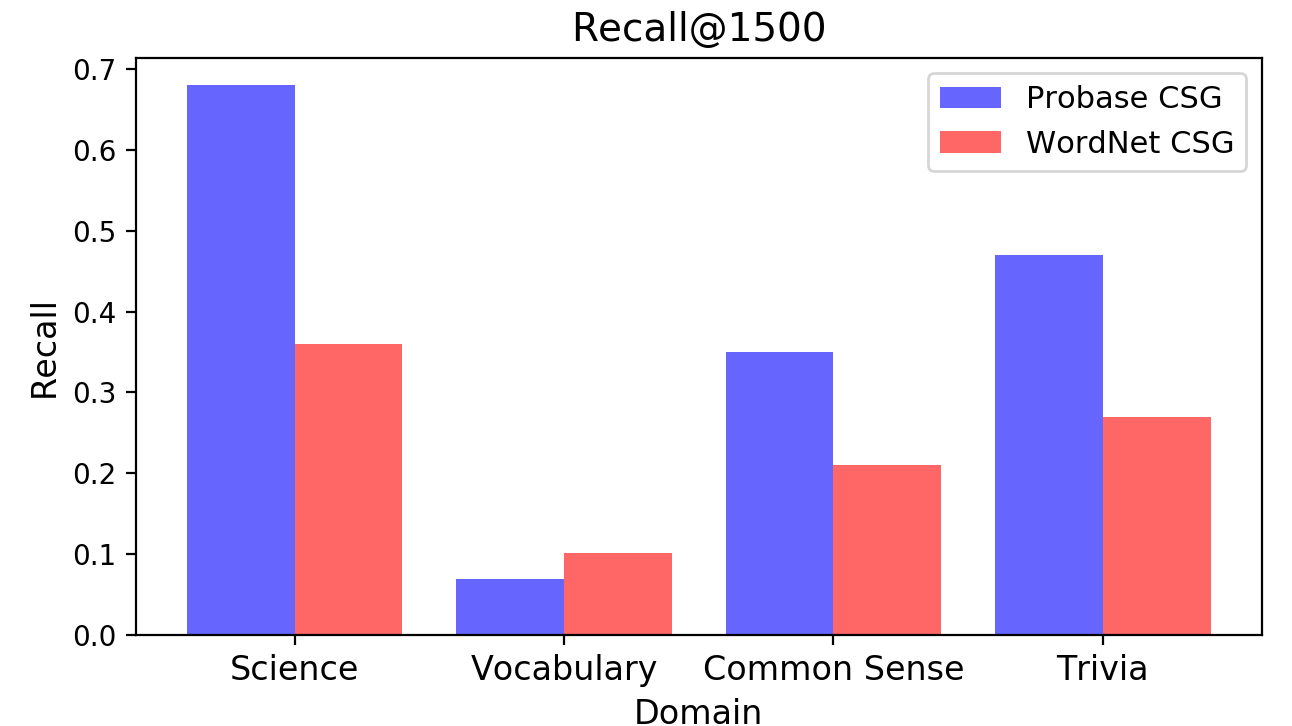
\includegraphics[width=1.0\columnwidth]{figure/recall.png}}
% 	\caption{Recall@1500 of Probase CSG and WordNet CSG in different domains.} \label{fig:recallk}
% \end{figure}

% \begin{table}[htb!]
% 	\small
% 	\centering
% 	\begin{tabular}{|c|c|c|c|c|}
% 		\hline
% 		K &  50 & 500 & 1000 &  1500 \\
% 		\hline
% 		WordNet CSG & 11.9\% & 23.5\% & 25.7\% & 26.5\%\\
% 		\hline
% 		Probase CSG & \textbf{22.8}\% & \textbf{39.3}\% & \textbf{45.1}\% & \textbf{47.8}\%\\
% 		\hline
% 	\end{tabular}
% 	\caption{Recall@K of WordNet CSG and Probase CSG without DS. Results are averaged across all domains.}
% 	\label{table:recall}
% \end{table}


% \begin{figure}[h!]
%   \centering
%   \subfigure[F1@3 score in different domains.]{
%     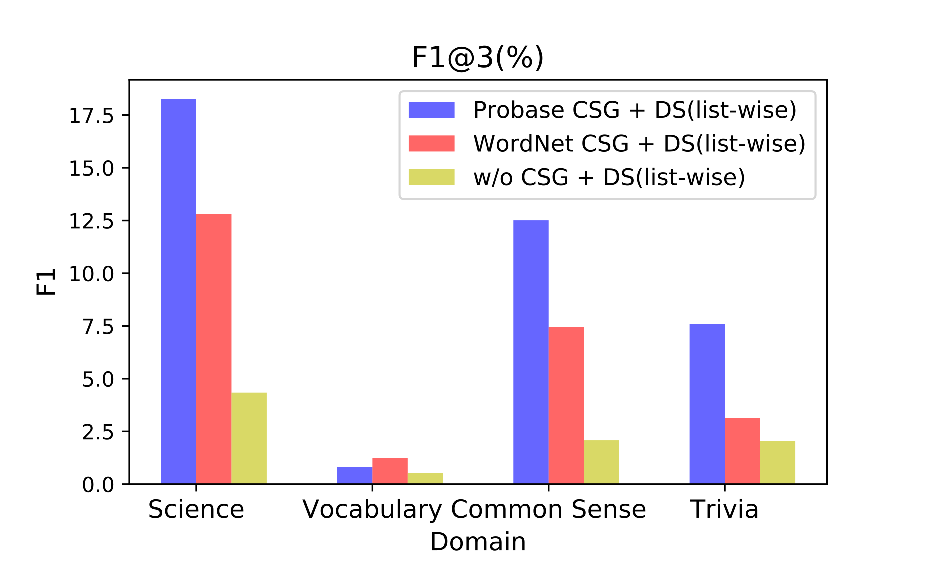
\includegraphics[width=0.35\textwidth]{figure/f1.eps}}
%   \hspace{1in}
%   \subfigure[NDCG@10 score in different domains.]{
%     \includegraphics[width=0.35\textwidth]{figure/ndcg.eps}}
%   \caption{F1@3 and NDCG@10 in different domains.}
%   \label{fig:domains} %% label for entire figure
% \end{figure}

\noindent
\textbf{Domain Effect \& Feature Importance.} ~\figref{fig:domains} shows the F1@3 of CSG+DS in different domains. The performance drops most drastically when applied in vocabulary domain because adjectives and adverbs in Probase and WordNet are either rare or not hierarchically organized. Another possible explanation is that the ground truth distractors in vocabulary domain are less semantically-related to the key, which makes learning process of the ranker oscillatory.
Our framework is especially better at generating distractors in science and commonsense domain, in which the keys and distractors are mostly subject-specific~(e.g. physics) terminologies, real-world entities and other common nouns. Trivia domain has similar characteristic but the keys are often rarer, therefore Probase suffers less due to its larger scope.
To have more insights on the proposed features, we also conduct feature importance analysis of DS based on mean reduced impurity. It is defined as the total decrease in node impurity, weighted by the probability of reaching that node, averaged over all base classifier. \tabref{table:feat_importance} reveals that semantic relation between $a$ and $d$ and web search score play more critical role than features of other aspects.
\label{sec:endtoend}

\begin{table}[t]
			\centering
		\small
		\addtolength{\tabcolsep}{-2pt}
		\begin{tabular}{c|c}
		\toprule
		Probase CSG & WordNet CSG \\

			\midrule
		contextual embed sim(a,d) & contextual embed sim(a,d) \\
		 word2vec embed sim(a,d)   & word2vec embed sim(a,d)  \\
		  word2vec embed sim(q,d)& word2vec embed sim(q,d)  \\
		  web search score & web search score \\
		  relative LCS len(d)   & relative LCS len(d)  \\
		  relative LCS len(a)  & relative LCS len(a)  \\
		  character len(d)   & character len(d)  \\
		  character len difference(a,d)   & character len difference(a,d)  \\
		  edit distance(a,d)   & edit distance(a,d)  \\
		  POS similarity(a,d)   &  relative common suffix len(a) \\
		\bottomrule
	\end{tabular}
	\caption{Top 10 important features of list-wise DS.}
	\label{table:feat_importance}
\end{table}
\begin{table*}[t!]
	% \footnotesize
	\small
	\centering
		\begin{tabular}{lc cc c c c c c cc}
			\toprule
			\multirow{3}{*}{\textbf{Method}} &\multicolumn{2}{c|}{\textbf{Human Evaluation}} &\multicolumn{7}{c}{\textbf{Automatic Evaluation}} \\
			\\ [-1.8ex]
			\cline{2-10}
			\\ [-1.8ex]
			& Reliability & Plausibility  &F1@3 & P@1 & P@3 &R@3 & MRR & NDCG@10 & \tabincell{c}{Semantic \\ Similarity@3}\\
			\midrule
			TM &95.57\%  &1.25$\pm$0.41 &1.74 &0.40  &1.16  &3.48   &2.69  &4.79  &0.21 \\
			\midrule
			\textbf{WordNet CSG} &98.66\% &1.25$\pm$0.34 &3.14 &3.49 &2.33 &5.43 &7.19 &8.66 &0.26 \\
			+~ED &90.66\% &1.26$\pm$0.41  &0.41 &0.12  &0.26  &0.58  &2.10  &1.93  &0.20 \\
			+~RevUP &93.65\%  &1.22$\pm$0.34  &4.07 &5.79  &3.21  &6.43 &9.31  &9.60  &0.32 \\
			+~EmbSim+CF &\textbf{99.12}\%  &1.21$\pm$0.49  &4.62  &6.17  &3.60  &7.40  &10.32  &10.94  &0.36 \\
			+~BERT &89.94\% &1.23$\pm$0.58  &5.68 &6.93  &4.23  &9.57  &11.10  &11.66  &0.30 \\
			+~LR+LM &96.66\%  &1.25$\pm$0.35 &6.48 &9.25  &4.89 &10.81   &13.42 &13.66 &0.29\\
			+~LR+RF &95.56\%  &1.25$\pm$0.38 &6.67 &8.10 &5.14 &10.81   &13.18 &13.73 &0.30 \\
			+~\textbf{DS(lise-wise)} &98.66\%  &\textbf{1.35$\pm$0.40}   &\textbf{7.71} &\textbf{9.31} &\textbf{5.81} &\textbf{12.98} &\textbf{14.34} &\textbf{14.94} &\textbf{0.36} \\
			\midrule
			\textbf{Probase CSG} &99.23\% &1.26$\pm$0.35 &5.88 &6.98 &4.39 &9.95  &12.07 &13.40 &0.34 \\
			+~ED &94.33\%  &1.23$\pm$0.38  &0.82 &1.16  &0.65  &1.30  &5.02  &4.92  &0.28 \\
			+~RevUP &94.87\%  &1.26$\pm$0.36  &6.27 &5.40  &4.63  &10.68  &11.74  &14.23  &0.37 \\
			+~EmbSim+CF &96.98\%  &1.19$\pm$0.47  &7.01 &8.10  &5.14  &12.34  &13.86  &16.33  &0.41 \\
			+~BERT &95.00\% &1.27$\pm$0.58  &7.05 &7.72  &5.14  &12.23  &13.60  &16.21  &0.36 \\
			+~LR+LM &98.98\%  &1.25$\pm$0.30   &7.62  &8.53  &5.81 &12.27 &15.56 &16.83 &0.40 \\
			+~LR+RF &99.13\%  &1.24$\pm$0.31   &7.48 &8.52 &5.42 &13.17   &15.87 &19.03 &0.40\\
			+~\textbf{DS(list-wise)} &\textbf{99.33}\%  &\textbf{1.30$\pm$0.34} &\textbf{9.19}  &\textbf{10.85} &\textbf{6.72} &\textbf{15.88} &\textbf{17.51} &\textbf{19.31} &\textbf{0.41} \\
			\midrule
			\textbf{w/o CSG} &- &- &- &- &- &-  &- &- &- \\
			+~ED &93.98\%  &1.00$\pm$0.12  &0.19 &0.38  &0.12  &0.38  &0.54  &0.53  &0.11 \\
			+~RevUP &92.88\%  &1.02$\pm$0.14  &2.01 &2.35  &1.35  &4.21  &3.95  &5.12  &0.38 \\
			+~EmbSim+CF &94.77\%  &0.93$\pm$0.52  &2.12 &2.70  &1.41  &4.24  &4.19  &5.24  &\textbf{0.42} \\
			+~BERT &93.87\% &1.02$\pm$0.24  &3.03 &2.88  &2.15  &5.14  &5.29  &6.78  &0.39 \\
			+~LR+LM &96.77\%  &1.05$\pm$0.28   &4.22  &4.34  &2.79 &8.69 &7.02 &10.16 &0.41 \\
			+~LR+RF &97.78\%  &1.02$\pm$0.20   &4.05  &4.21 &2.66 &8.55 &6.91 &10.08 &0.40\\
			+~\textbf{DS(pair-wise)} &\textbf{98.43}\%  &\textbf{1.06$\pm$0.14} &\textbf{5.59} &\textbf{5.01} &\textbf{3.98} &\textbf{10.10}  &\textbf{9.28} &\textbf{11.60} &0.36\\
			\midrule
			ground truth &\textbf{100\%}  &\textbf{1.41$\pm$0.35}  & - & - & - & - & - & - & -\\
			\bottomrule
		\end{tabular}
		\caption{End-to-end comparison on test set. - means no ranking algorithm to evaluate and ``ground truth'' denotes the score of ground-truth distractors associated with each item.}
		\label{table:human}
	\end{table*}
	\begin{table*}[t!]%[th]
		\small
		\centering
			\begin{tabular}{cccccccc} %/tabincell{c}{haha// heihei//zeze}
				\toprule
				 \textbf{Key} &RevUP &ED  & EmbSim+CF &BERT & LR+RF & LR+LM & \textbf{DS}\\
				\midrule
				  \color{red} \textbf{0.42} &0.06  &0.03  &0.04 &0.12  &0.11 &0.07   &\textbf{0.14}\\
				\midrule
			\end{tabular}
			\caption{Human evaluation on the frequency of being chosen as answer for each model paired with Probase CSG. DS denotes our list-wise distractor selector. Red colored number corresponds to the correct answer.} 
			\label{table:app}
		\end{table*}
\noindent

\textbf{End-to-End Comparison.} ~\tabref{table:human} shows the end-to-end results.
Despite the significantly reduced number of candidates, ranking methods with our candidate set generator can achieve much higher performance than with unstructured vocabulary. TM performs poorly due to its naive path similarity ranking criterion. The results of ED are worst among all unsupervised methods while embedding based methods can even achieve comparable performance against LR+LM/RF when provided with a high-quality candidate set.
BERT ranks distractors using contextualized representation thus leading to lowest reliability according to human evaluation. 
LR+RF/LM achieves similar ranking performance yet obtain poorer reliability than CSG+DS since they only focus on the plausibility of selected distractors. CSG+DS, despite its relative simplicity, obtain consistent improvements over LR+RF/LM without two-stage cascaded training.
We observe certain inconsistency between plausibility and automatic metrics of baselines, part of the reason may be that methods such as LR+RF/LM focus much on shallow feature patterns of ground-truth distractors and fail to unearth potential acceptable distractors.
However, distractors generated by CSG+DS yield highest ranking measures while rated as most plausible by human annotators. 
Unsupervised methods work solely relying on the semantic similarity hence their reliabilities are generally lower than supervised ones, among which our DS turns out to be the most reliable. Exceptionally, EmbSim+CF gets higher reliability with WordNet, whose unreliable candidates get more chance to be eliminated by post-filtering than those in Probase.

\noindent
\textbf{Application-Centric Evaluation.} ~The frequency of generated distractors being chosen as answer for each tested model is shown in \tabref{table:app}. Our DS obtains the highest distracting rate compared to all baselines, indicating that distractors generated by our framework is more likely to distract testees in real world scenarios. The pearson correlation coefficient between the frequency and F1@3 is 0.46, implying certain positive correlation between automatic metrics and actual distracting capacity.




% Distractors generated by CSG+DS have very competitive quality, scoring on average 1.12, even higher than the average score of the ground truth designed by human experts. They are also less likely to be rated ``Obviously Wrong.'' 
% The reason is that, different from other methods, 
% CSG+DS method can make full use of the rich information in the stem 
% to generate distractors belonging to the same concept-level as the key 
% with contextual fit, which is also challenging for human experts. 
% For example, for the stem ``\textit{\underline{\hbox to 8mm{}} functions primarily to defend the body against disease.}'' and the key ``\textit{immune}'', our CSG+DS method generates ``\textit{reproductive, respiratory, digestive}'' which belong to the same concept \textit{functions} as the key. On the other hand, the ground truth distractor \textit{nervous} is not similar to the key enough. TM and WP achieve low plausibility since it does not consider latent context, leading to many obviously wrong distractors. Although WP does make use of context words, it treats the key and other context words similarly and may select distractors similar to a context word instead of the key.  

% CSG+DS shows a significant improvement in reliability compared with baselines. TM, with 83.96\% reliability, is more prone to yield invalid distractors that are correct answers. This is not unexpected since it tries to find distractors from synonyms of the key, which are likely to have exactly the same meaning as the key.
% However, CSG+DS retrieves candidates belonging to the same concept-level, thus generate less invalid distractors. We also find that, with the same CSG, adding DS component helps improve the reliability rate, which verifies the effectiveness of our reliability checking features.
% {Case Study \& Discussion}

% \begin{table*}[htb!]
% 	\small
% 	\centering
% 		\begin{tabular}{|l|c c c c c c c |c|}
% 			\hline
% 			\multirow{3}{*}{Method} &\multicolumn{7}{|c|}{Automatic Evaluation(\%)} \\
% 			\cline{2-8}
% 			&F1@3 & P@1 & P@3 &R@3 & MRR & NDCG@10 & \tabincell{c}{Semantic \\ Similarity@3}\\
% 			\hline
% 			\textbf{WordNet Vocab} &- &- &- &-  &- &- &- \\
% 			+~RevUP  &0 &0  &0  &0  &0  &  & \\
% 			+~EmbSim+CF  & &  &  &  &  &  & \\
% 			+~ED & &  &  &  &  &  & \\
% 			+~BERT & &  &  &  &  &  & \\
% 			+~LR+LM &  &  & & & & & \\
% 			+~LR+RF & & & &   & & &\\
% 			+~\textbf{DS(list-wise)} &\textbf{}  &\textbf{} &\textbf{} &\textbf{} &\textbf{} &\textbf{} &\textbf{} \\
% 			\hline
% 		\end{tabular}
% 		\caption{Results by replacing CSG with vocabulary extracted from WordNet.}
% 		\label{table:ablation}
% 	\end{table*}
\subsection{Case Study}
% \begin{table*}[ht!]
% 	\small
% 	\centering
% 		\begin{tabular}{|l|l|c c c c c c c|}
% 			\hline
% 			Method& Domain &F1@3 & P@1 & P@3 &R@3  & MRR & NDCG@10 & \tabincell{c}{Semantic \\Similarity@3}\\
% 			\hline
% 			\multirow{5}{*}{\tabincell{l}{WordNet CSG~+\\ list-wise ranker DS}} &Science &12.82  &21.73  &9.42 &21.73 &25.59 &23.29  &35.72 \\
% 			&Common Sense &7.45  &13.89  &5.56 &12.73 &15.80 &13.61 &27.45 \\
% 			&Vocabulary &0.43  &0.22  &0.28 &0.84  &0.72  &1.12  &24.18 \\
% 			&Trivia &3.13  &2.40  &2.61 &4.22 &7.61  &8.18  &24.99  \\
% 			\cline{2-9}
% 			&Total &7.71 &9.31 &5.81 &12.98 &14.34 &14.94 &34.68 \\
% 			\hline
% 			\multirow{5}{*}{\tabincell{l}{Probase CSG~+\\ list-wise ranker DS}} &Science &18.26  &28.26  &13.76 &30.43 &40.91  &38.35  &44.58 \\
% 			&Common Sense &12.51  &20.83  &10.19 &18.75 &27.28 &22.61 &33.47 \\
% 			&Vocabulary &0.41  &0.21  &0.27 &0.84  &0.58  &0.88  &12.75 \\
% 			&Trivia &7.59  &9.63  &6.42 &10.54 &20.39  &19.87  &34.49 \\
% 			\cline{2-9}
% 			&Total &9.19 &10.85 &6.72 &15.88 &17.51 &19.31 &40.71\\
% 			\hline
% 		\end{tabular}
% 		\caption{Results(\%) of the two best performing CSG+DS instantiations in different domains.}
% 		\label{table:domains}
% 	\end{table*}
\begin{table*}[ht!]%[th]
	\small
	\centering
		\begin{tabular}{lcccccccc} %/tabincell{c}{haha// heihei//zeze}
			\toprule
			\# &-  &RevUP &ED  & EmbSim+CF &BERT & LR+RF & LR+LM & \textbf{DS}\\
			\midrule
			1 &\color{red}protein   &\color{red}protein  &aldehydes  &starch &glycosaminoglycans  & hydrocarbon &methane    &\color{red} fat\\
			\midrule
			2 &alcohol  &alcohol  &carboxylic acid  &glycerol  &glycerol &methane  &\color{red}protein    &\color{red}protein \\
			\midrule
			3 &benzene  &amino acid  &alcohol   &\textbf{glucose}  &aldehydes &hormone  &hormone   &peptide \\
			\bottomrule
		\end{tabular}
		\caption{Top 3 distractors from different ranker running with Probase CSG(- denotes sole Probase CSG)
	given the stem ``The main source of energy for your body is \underline{\hbox to8mm{}}.'' and the key ``{\color{blue}carbohydrate}''. Red colored distractors are the ground truth, bold distractors are unreliable distractors.}
		\label{table:example}
	\end{table*}
\tabref{table:example} compares predictions made by all baselines and DS~(list-wise) running with Probase CSG. We can see that Probase CSG alone and RevUP are both able to generate distractors belonging to the same concept level as the key and accurately match one ground truth. However, running Probase CSG with ED yields 
distractors that are more semantically distant from the key. 
Despite the use of candidate filtering, EmbSim+CF still produces candidates 
like ``glucose'', which is an eligible answer to the stem. 
BERT instead generate compound names that are too technical and belong to lower concept level than ground truth. 
Among all the supervised rankers, DS hits another ground-truth distractor 
``fat'' while LM+RF/LM predict some obviously wrong distractors 
such as ``methane'' due to its coarse-grained features.


% We refer readers to supplementary metrial for more sample distractors generated by different methods.
